\section{Continuations with Effects}
\TableOfContents{}

\subsection{Why continuations for effects?}
\begin{frame}
	\frametitlesubs{}

	{
		\only<.(3)->{\smaller[2]}
		\textit{Effects}, side effects or computational effects:
		\vspace*{-1.1\zh}

		\begin{center}
			\begin{minipage}[t]{.7\textwidth}
				\begin{itemize}
					\only<.(3)->{\setlength{\itemsep}{-.2\zh}}
					\item Exception {\only<.(2)->{\dotfill \textit{halt?}}}
					\item Async I/O {\only<.(2)->{\dotfill \textit{when to resume?}}}
					\item Coroutines {\only<.(2)->{\dotfill \textit{which order to resume?}}}
					\item etc.
				\end{itemize}
			\end{minipage}
		\end{center}
	}

	\vspace{.2\zh}
	Handling effects is about what happens------
	\pause
	\\\centerline{\larger{}and \textit{when} and \textit{how} to \textcolor{subhighlight}{resume}.}

	\pause

	\vspace{-.4\zh}
	\centering
	\hspace*{\fill}
	\begin{minipage}[t]{.41\textwidth}
		\vspace{.6\zh}

		\centering
		\large
		So, it's time
		for
		\LARGE
		\textcolor{highlight}{\boldslant Continuations!}
	\end{minipage}
	\begin{minipage}[t]{.30\textwidth}
		\begin{figure}[h]
			\centering
			\sloppy
			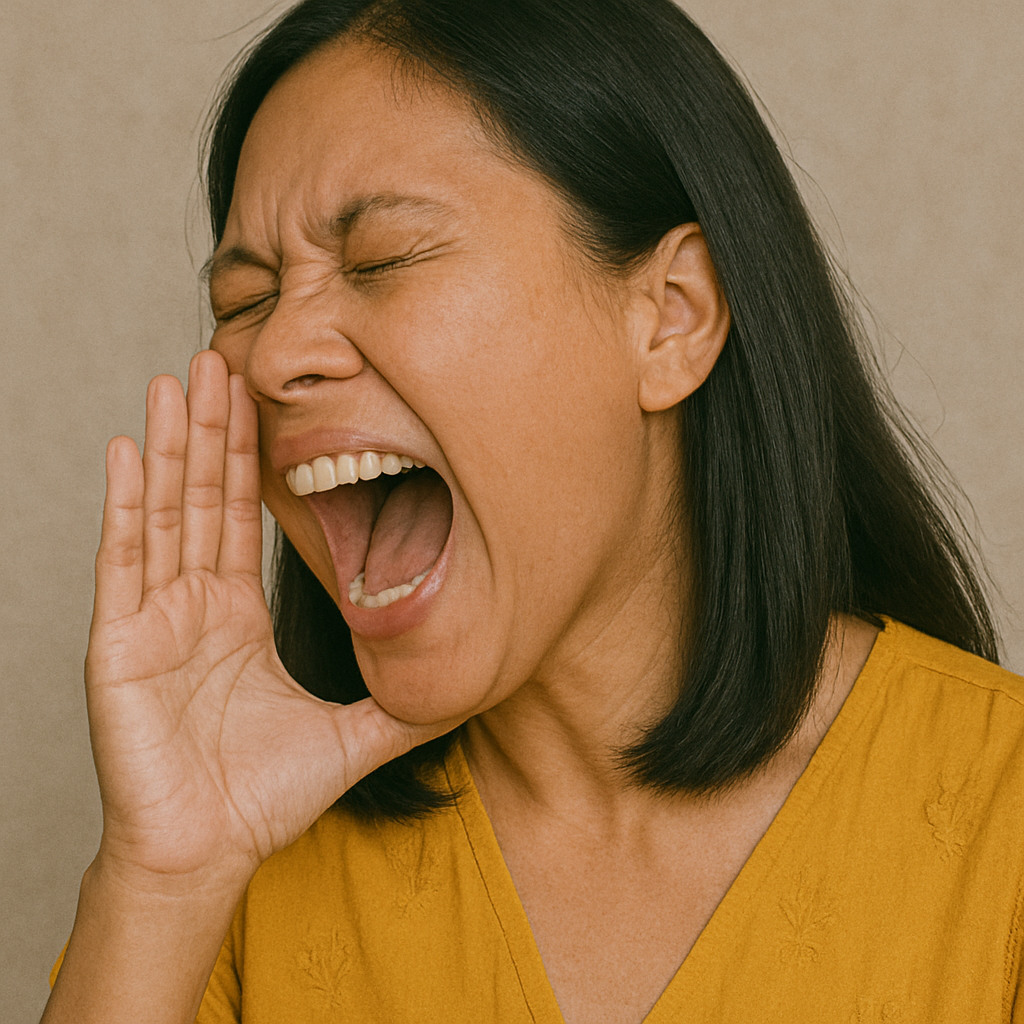
\includegraphics[height=.38\textheight]{img/woman-shouting.png}
		\end{figure}
	\end{minipage}
\end{frame}

\subsection{Monads}

\begin{frame}[fragile]
	\frametitlesubs{}

	An approach to modeling calculi with \textit{effects}\cite{moggi1991notions}:

	\begin{center}
		\begin{minipage}{.63\textwidth}
			\begin{minted}{haskell}
        class Monad m where
          return :: a -> m a
          (>>=)  :: m a -> ?\tikzmarknode{bindk}?(a -> m b) -> m b?\tikzmarknode{bindke}?
      \end{minted}
		\end{minipage}
	\end{center}

	\pause
	\begin{tikzpicture}[overlay]
		\path[draw, line width=1.5pt, color=highlight] ([yshift=-.2\zh]bindk.south) edge node[midway,above=0.4]{\footnotesize continuation} ([yshift=-.2\zh]bindke.south);
	\end{tikzpicture}

	\pause
	\centering

	\setminted{fontsize=\footnotesize}
	\begin{minipage}{.4\textwidth}
		\begin{minted}{haskell}
      instance Monad Maybe where
        return = Just
        Just x  >>= k = k x
        Nothing >>= ?\tikzmarknode{nothing}{\texttt{\_}}? = Nothing
    \end{minted}
	\end{minipage}
	\hspace{.1\textwidth}
	\begin{minipage}{.3\textwidth}
		\pause

		\begin{minted}{haskell}
      maybe e >>= \x -> u
    \end{minted}
		\vskip-.1\baselineskip

		\pause

		\centering
		\begin{tabular}{rl}
			$\Downarrow$ &
			\smaller[2]
			\begin{tabular}{c}
				direct-style \\
				with \texttt{do}
			\end{tabular}
		\end{tabular}
		\vskip-.1\baselineskip

		\begin{minipage}{.75\textwidth}
			\begin{minted}{haskell}
        do
          x <- maybe e
          u
      \end{minted}
		\end{minipage}
	\end{minipage}

	\pause

	\begin{tikzpicture}[overlay]
		\node at (nothing) {\LARGE\textcolor{highlight}{\bf\_}};
		\node[below = .2 of nothing, rotate=-20] {\Huge\emoji{backhand-index-pointing-up}};
		\node[below right = .2 of nothing, yshift=-.7\baselineskip] {
			\small
			\begin{tabular}{l}
				\textcolor{highlight}{throw away} continuation \\
				to stop computation\textbf{!}
			\end{tabular}
		};
	\end{tikzpicture}
\end{frame}

\subsection{Algebraic Effect Handlers}
\begin{frame}[fragile]
	\frametitlesubs

	A new way to model effectful computations, with high \textit{modularity} and \textit{composablility}\cite{bauer2013effect}:

	\vskip-.2\baselineskip
	\begin{center}
		\begin{minipage}{.7\textwidth}
			\begin{minted}{ocaml}
        type _ eff += Print : string -> unit eff

        match perform @@ Print "hello" with
        | effect (Print msg), ?\textcolor{highlight}{\bf\tt k}? ->
          print_endline msg; ?\textcolor{highlight}{\bf\tt continue k ()}?
      \end{minted}
		\end{minipage}
	\end{center}

	\pause

	\begin{center}
		\vspace*{-.1\baselineskip}
		\begin{minipage}[t]{.44\textwidth}
			\centering
			\parbox[c][.35\textheight][c]{\textwidth}{
				\begin{center}
					\textcolor{subhighlight}{Handlers} make it \textit{easier} to \textbf{compose} and \textbf{modularise}

					than

					\textcolor{highlight}{monad transformers}\textbf{!}
				\end{center}
			}
		\end{minipage}
		\hspace{.03\textwidth}
		\begin{minipage}[t]{.4\textwidth}
			\parbox[t][.3\textheight][t]{\textwidth}{
				
\includegraphics[width=3.6\zw]{img/notgood.png}\raisebox{2\zh}{\tiny\footnote{\url{https://www.youtube.com/watch?v=uxpDa-c-4Mc}}}
				\raisebox{1.2\baselineskip}{\mbox{
						\footnotesize
						\color{highlight}
						\begin{tabular}{c}
							Monad \\
							Transformers
						\end{tabular}
					}}
				\vskip-.4\baselineskip

				
\includegraphics[width=3.6\zw]{img/good.png}
				\raisebox{\baselineskip}{\mbox{
						\footnotesize
						\color{subhighlight}
						\begin{tabular}{c}
							Algebraic Effect \\
							Handlers
						\end{tabular}
					}}}
		\end{minipage}
	\end{center}
\end{frame}
